\chapter{Implementation}

\paragraph{} This chapter shall first explain how turtles are defined along with the remaining features of the initial prototype. The format and results of the formative evaluation using this initial prototype shall be summarised. I shall then cover the design decisions and changes that were made to the Excello prototype during this participatory design process. Then, the technical details of Excello and the MIDI to Excello converter will be covered. Concluding with an overview of the project repository.

\section{Initial Prototype}

\paragraph{} Notes and turtles can be defined in any cell. The interpretation of cell contents by turtles is shown in table \ref{tab:cells}. When the Excello add-in is opened, a window will open in the right side of Excel. A play and stop button can be used to launch all the turtles defined in the spreadsheet and initiate playback. Playback is a realistic piano sound.

\begin{table}
\centering
% \caption{Grammar Rules for the turtle movement instructions. $z \in \Z$}
\caption{Definition of notes in cells.}
\vspace{1pt}
\begin{tabular}{|l|l|} \hline
\textbf{Interpretation}&\textbf{Format}\\ \hline
Note& Note name (A-G), optional accidentals and octave \\
&number e.g. \texttt{F\#4}\\ \hline
Sustain& \texttt{s}\\ \hline
Multiple notes& Notes, rests or sustains separated by a comma. Rests \\
subdivided in time& must be a space or an empty string e.g. \texttt{E4,,C4,s}\\ \hline
Rest& Any cell not interpreted as a note, sustain or multi-note. \\ \hline
\end{tabular}
\label{tab:cells}
\end{table}

\subsection{Turtles}

\paragraph{} Turtles are defined as follows:

\texttt{!turtle(<Starting Cell>, <Movement>, <Speed>, <Number of Loops>)}

\subsubsection{Activation}

\paragraph{} "\texttt{!}" dictates that the turtle will be activated when the play button is pressed. Just as digital audio workstations allow muting and soloing of tracks, this can be used to quickly modify which turtles will play without losing their definitions.

\subsubsection{Starting Cell}

\paragraph{} The starting cell of the turtle, which is also played, is given by the cell reference. As with Excel formulae, this is a concatenation of letters for the column and numbers for the row.

\paragraph{} As each turtle only plays one note at a time, multiple turtles must be defined to play polyphonic music such as chords. It was believed that user would define turtles following identical paths but in adjacent rows or columns. Multiple turtles following identical paths but starting from adjacent cells can be defined using the existing Excel range notation for the starting cells. "\texttt{A2:A5}" would define four turtles in the cells A2,A3,A4,A5. This prevents the writing of multiple turtle definitions differing in only the start cell row.

\subsubsection{Movement}

\paragraph{} Turtles start facing north. The language for programming turtle movement has been discussed in the preparation chapter. Using brackets to repeat movements within the turtle's instructions was not implemented by the start of the participatory design process.

\subsubsection{Speed}

\paragraph{} An optional third argument declares the speed the turtle moves through the grid relative to 160 cells per minute. The default is 1 corresponding to 160 cells per minute. If the argument "\texttt{2}" was provided, this would move through the grid at 320 cells per minute. This relative system was used so it would be easier to tell the speed relation between two turtles. This would be particularly beneficial for phase music. Arbitrary maths can be provided for this argument allowing turtles' speeds to be irrational multiples of each other.

\subsubsection{Number of Loops}

\paragraph{} An optional fourth argument defines the number of repetitions of the turtle's path. By default, the turtle will loop infinitely. This was included so that repeating parts (e.g. the cello  of Pachabel's Canon in D) need only defining once.

\subsection{Highlighting}

\paragraph{} To assist in the recognition of notes and turtles, when the play button is pressed, cells are highlighted, conditional on their contents. Cells containing activated or deactivated turtle definitions are highlighted green. Cells containing definitions of notes, or multiple notes, are highlighted red. Sustain cells are highlighted a lighter red, to show a correspondance to notes whilst maintaining differentiation.

\subsection{Chord input}

\paragraph{} In order to use musical abstractions of chords and arpeggios\footnote{Where the notes of a chord are played in rising or descending order} whilst keeping the paradigm of a turtle being responsible for up to one note at any time, a tool to add them is included. The note, type, inversion and starting octave of the chord are inputted in four drop-down selectors and the insert button enters the notes making up that chord into the grid. If a single cell or range taller than it is wide is highlighted in the spreadsheet, the notes will be inserted vertically starting at the top-left of the range. Otherwise, the notes will be inserted horizontally. This means whether the turtles are moving horizontally or vertically both chords and arpeggios can be easily defined. Thus, helpful musical abstractions are still available whilst keeping the cleanness of the turtle system.

\section{Formative Evaluation}

\paragraph{} To guide development to best suite users, participants were involved in formative evaluation. 21 participants took place in the participatory design process. Participants were all musical University of Cambridge students, across a range of subjects. Initially, one-on-one tutorials of the initial prototype were given followed by the user carrying out of a short exercise. After both the tutorial and the exercise, users were interviewed on how they found Excello, drawing particular attention to actions that they found particularly unintuitive or requiring notable mental effort. Comparisons were made to the musical interfaces that participants were already familiar with. The sessions were audio recorded in order to prevent the jotting down of notes causing delays. Notes were later made from these recordings. The ethical and data handling procedures shall be discussed in the evaluation chapter.

\paragraph{} For realistic simulation of the ways in which Excello would be used, participants were given the freedom to carry out an exercise of their choice. In many cases this was transcribing an exiting piece from memory or traditional western notation into the Excello notation. Two tasks were provided to choose from if participants had no immediate inspiration; transcribing a piece of western notation music or making changes to existing Excello notation.

\paragraph{} These sessions were carried out at the beginning of Lent term 2019. Participants were asked if they would be willing to continue using Excello personally until the summative evaluation sessions, eight weeks later. This allowed additional feedback to be given as participants used Excello in their own time. It also ensured that the summative evaluation would be done using users with sufficient experience of the interface.
% Participants were encouraged to get in contact with any additional issues or suggestions they had during this time.

\subsection{Issues and Suggestions}

\paragraph{} The issues and suggestions from the participatory design process have been summarised below.

\subsubsection{Turtle Notation}

\paragraph{} Dynamics in the turtle instructions made it harder to extract the turtle's path as not all instructions related movement. As the dynamics weren't next to the notes they corresponded to, it was challenging to know the of volume a note or where to place the dynamics within the turtle to affect a certain note elsewhere in the spreadsheet. The initial prototype had no way to assign a dynamic to the first note without having the starting cell being empty. This empty cell could be inconvenient for looping parts as it would be included in the loop. Users not familiar with the dynamics of western notation found them unintuitive. Furthermore, these discrete markings do not make available the continuous volume scale possible with the interface.

\paragraph{} When transcribing a piece with exact tempo, dividing the speed by 160 to enter the relative speed caused unnecessary work. There was also forgetfulness as to whether relative speed referred to how long the turtle spent in each cell or how quickly the turtle moved. Having completed the tutorial, users often had to check the position and meaning of turtle arguments.

\paragraph{} As the number of dynamics and movement instructions grew, the instructions became long and it could be tough to parse and then establish turtle behaivour. Also, becuase "\texttt{s}" could be used to indicate sustain within cells, some users confused the "\texttt{s}" within the turtle instructions to mean sustain and not south.

\subsubsection{Feedback}

\paragraph{} It was often unknown if pressing play registered, especially if the Excel workbook was saving delayed Excello being able to access the spreadsheet. Users also requested to see a summary of where the active turtle were in addition to the highlighting. If a turtle had accidentally been left activated, the entire grid had to be searched in order to locate it.

\subsubsection{MIDI conversions}

\paragraph{} Many users who use production software said importing and exporting MIDI files would be helpful. If working with an existing MIDI file, it would be convenient to be able to convert that into the Excello notation. Exportation would allow Excello to be used to create chord sequences, bass lines and the piece structure, before adding additional effects and recorded lines in their digital audio work stations.

\subsubsection{Sources of effort when writing}

\paragraph{} Once notes had been inputted into the grid, the number of cells the turtle had to move had to be counted. This is often in a straight line. Whilst the Excel status bar allows users to highlight a selection of cells and immediately see how many cells are highlighted, this is unproductive. This was particularly inconvenient when users were writing out a piece and periodically testing what they had written so far. Some users simply instructed turtles to move forward significantly more steps than required to prevent this counting. This is not feasible for looping parts. It was suggested that turtles figure out how far they should move.

\paragraph{} Instructions involving repeated movements such as moving to the end of a line and jumping down to the beginning of a line below, instructions within the turtles required a lot of repetition.

\paragraph{} Many of the notes in melodic lines would take place in the same octave. As such, repeatedly writing out the octave number was tiresome. One user made a comparison to LilyPond \cite{sandberg:lily} where if the length of a note is not defined, the last defined note length would be used.

\paragraph{} Some users find it more intuitive to think of a melodic line as the intervals between notes as opposed to note names. A modulated\footnote{Where every note has been moved up or down in pitch by the same amount.} melody line required the modulated part to be written out again and could not be derived quicker from the original version.

\subsubsection{Chords}

\paragraph{} Most users used a very small subset of the available chords but had to scroll through the whole list to find these. Separating the more common chords for easier access was requested. Initially, notes inserted vertically  had the lowest note at the top with notes increasing in pitch proceeding down the column. In western staff notation, higher pitch notes appear higher up the staff. As a result, it was suggested that inverting the order would be more intuitive. In the initial interface it was also unclear what the different drop downs corresponded to, with some users selecting the 7 from the octave number in order to try and insert a Maj7 chord.

\subsubsection{Activation of turtles}

\paragraph{} When toggling the activation of a turtle, entering the edit mode for each cell containing a turtle definition to add or remove the exclamation mark was very tedious.

\section{Second Prototype}

\paragraph{} Following the formative evaluation sessions and feedback, a series of additions and modifications were made to solve the problems and opportunities brought up.

\subsection{Dynamics}

\paragraph{} To help extract the path that the turtles follow and pair notes with their volume, dynamics are instead inserted in the cells along with the notes. A dynamic instruction is added after the note, separated by a space as in Manhattan \cite{nash:manhattan}. As before, this will persist for all following notes until the volume is redefined. A single turtle definition with multiple start cells can now play parts of different volume. However, notes in the grid are limited to only being played at their given volume. To play the same notes at a different volume, a new path must be made where the cells defining the volume are replaced. Overall, the new system was believed to be more preferable.

\paragraph{} In order to be able to make use of a full continuous dynamic scale, in addition to the existing dynamic symbols, a number between 0 and 1 can be provided where 0 will be silent and 1 is equivalent to fff.

\subsection{Nested Instructions}

\paragraph{} Nested instructions with repetitions reduces the length of turtle instructions and allows for repeated sections or movements to be more easily incorporated. A series of instructions placed within parentheses with a number immediately following the closing parenthesis will be repeated that number of times. Whilst the fourth argument of the turtle will simply repeat the entire musical output of the turtle, repetitions within the turtle instruction allow paths to be defined more concisely.

\subsection{Absolute Tempo}

\paragraph{} The turtle's speed is defined by cells per minute, rather than the relative value used initially. However, values less than 10 were interpreted in the original relative way to maintain backwards compatibility for the participant's existing work. To maintain consistency in a production version, this is removed so speed must be defined absolutely. The values given for speed and dynamics will be of different orders of magnitude and hence reduce the confusion that can occur between them.

\subsection{Custom Excel Functions}

\paragraph{} Two custom Excel functions were implemented to aid composition. One to insert turtles into the grid and a second to transpose notes.

\subsubsection{Excello.Turtle}

\paragraph{} By adding custom Excel functions, the existing formulae writing tools provided within Excel can be utilised. When using a built in formula, a prompt appears informing users which arguments go where and whether they are optional. The output of this function is text used to define a turtle if written manually. Other cells can be referenced for the arguments of the turtle function. For example all turtles could reference a single cell for their speeds. This allows relative tempos to be easily implemented as the speed argument of each turtle could be a relative speed mutliplied by this global speed as shown in figure \ref{implementation:turtleFunction}.

\begin{figure}[tbh]
\centerline{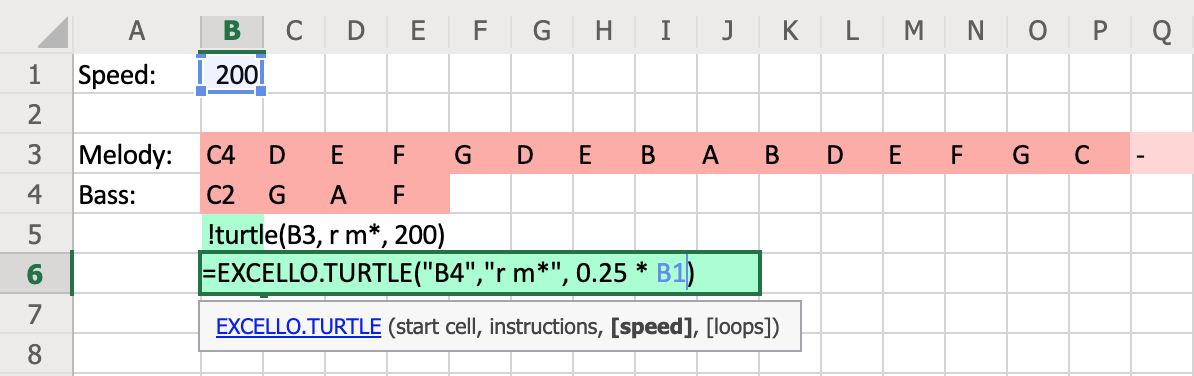
\includegraphics[width=150mm]{figs/turtleFunction.png}}
\caption{Defining a turtle using the EXCELLO.TURTLE function.}
\label{implementation:turtleFunction}
\end{figure}

\subsubsection{Excello.Modulate}

\paragraph{} A function to modulate notes provides easy modulation of existing sections of a piece and also the definition of a melodic line by the intervals between the notes. The function takes a cell and an interval and outputs any notes defined in that cell transposed by that interval, maintaining any dynamic definition. A section can be modulated by calling this function on the first note with a provided interval and using the existing drag-fill functionality of Excel to modulate all notes. By using the previous note that has just been transposed and one of a series of intervals as the arguments, a melodic line can quickly be produced from a starting note and a series of intervals as shown in figure \ref{implementation:modulateFunction}.

\begin{figure}[tbh]
\centerline{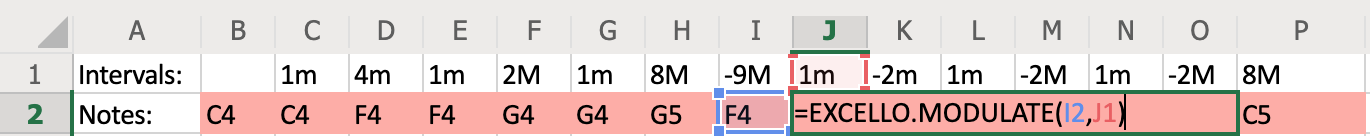
\includegraphics[width=150mm]{figs/modulateFunction.png}}
\caption{Transposing notes using the EXCELLO.MODULATE function.}
\label{implementation:modulateFunction}
\end{figure}

%  \ref{examples}

\subsection{Sustain}

\paragraph{} To prevent confusion between the instruction for a turtle to face south and sustains. The symbol "\texttt{-}" sustains a note. This was chosen because it is light and also has some similarity to a tie\footnote{A line to increase the length of a note by joining to another.}. "\texttt{s}" in a cell is still interpreted as a sustain to maintain backwards compatibility for the existing work of the participants.

\subsection{Active Turtles}

\paragraph{} In order to provide feedback that turtle definitions have been recognised, a list of the active turtles is given below the play button. This also helps find spurious turtles that were not intended to be activated.

\subsection{Automatic Movement}

\paragraph{} To prevent counting the number of cells in a line, \texttt{m*} instructs a turtle to move as far as there are notes defined in the direction it is currently facing. If more notes are added on this line, the turtle instructions do not need editing before pressing play. There may be cases where a part is meant to finish with a number of rests. As a rest is notated with a blank cell, a method of increasing the length of the path to include these rests is required. A cell can be explicitly defined as a rest with "\texttt{.}". This would be required if multiple turtles were defining a repeating section where one does not have the final cell of the section being a note, sustain or multi-note cell. Without an explicit rest the turtle would stop and repeat too soon and the parts would be out of phase.

\subsection{Inferred Octave}

\paragraph{} The octave number can be inferred by the program if omitted. Two methods were under consideration. Firstly, given that most intervals within music are small, the nearest note could be played.
% This means that a scale would only need the octave defining in the first note.
Whilst this method would likely require the least explicit statement of octave number it would be non-trivial to figure out the octave of a given note. The last defined octave in the path would need finding and then all subsequent notes walked through keeping track of the octave. The second consideration was to always use the last defined octave. Whilst this may require many octave definition around the boundary between octaves, it is easier to find what octave a note is played at as it is simply the last defined octave in the path. The second option was implemented.

\subsection{Chords}

\paragraph{} To aid entering common chords, common types are repeated in a separate group at the top of the type drop-down. The layout of the chord drop-downs was improved with labels added making it clearer what the values refer to. If the notes were entered vertically, the order was reversed to have a greater correspondence with traditional staff notation.

\subsection{Activation of turtles}

\paragraph{} A "Toggle Activation" button was added to the add-in window. When a cell or range is highlighted in the spreadsheet, the activation of any turtle definitions in this range will be toggled when the button is pressed.  This significantly increases the ease with which turtles can be seleted as only two clicks are required as opposed to having to enter the cell edit mode and add or remove an exclamation mark.

\section{Final Prototype Implementation}

\paragraph{} This section discusses the underlying implementation of the final prototype, following the participatory design. Excello consists of three main parts. The first, and largest, is the turtle system for playing the grid contents. The second is the method for inserting the notes of chords into the grid. Thirdly, turtle input and modulation is made available through the custom Excel functions.

\paragraph{} When the play button in the add-in window is pressed, the turtle definitions within the grid are identified. For each, the starting cell and movement instructions are used to establish the contents of the cells which it passes through. This is converted to a series of note definitions - pitch, start time, duration, volume. The speed and loop parameter are used to create the structure interpreted by the Tone.js library to schedule and initiate playback. An overview of the data flow and subtasks required to create the musical playback is show in figure \ref{fig:overview}.

\begin{figure}[tbh]
\begin{center}
  
  \tikzset{every picture/.style={line width=0.75pt}} %set default line width to 0.75pt

  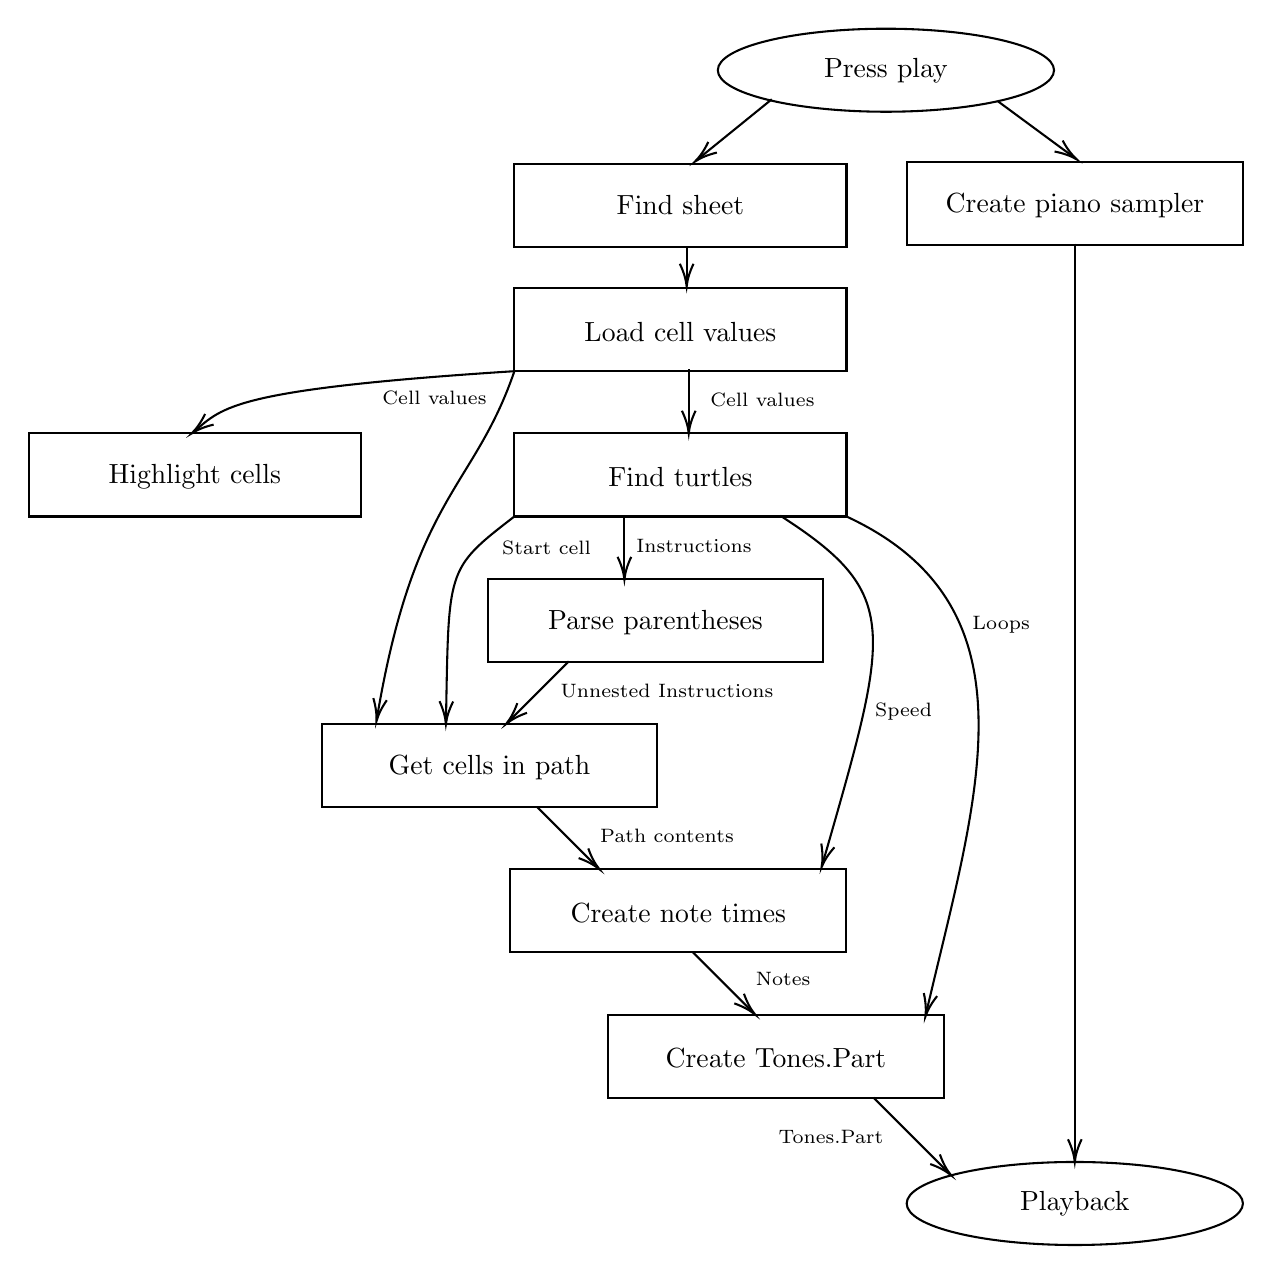
\begin{tikzpicture}[x=0.75pt,y=0.75pt,yscale=-1,xscale=1]
  %uncomment if require: \path (0,604); %set diagram left start at 0, and has height of 604

  %Shape: Rectangle [id:dp3390223975782729]
  \draw   (244.5,71) -- (404.5,71) -- (404.5,111) -- (244.5,111) -- cycle ;

  %Shape: Rectangle [id:dp7168559924493858]
  \draw   (244.5,131) -- (404.5,131) -- (404.5,171) -- (244.5,171) -- cycle ;

  %Shape: Rectangle [id:dp8835932361497658]
  \draw   (433.7,70) -- (595.5,70) -- (595.5,110) -- (433.7,110) -- cycle ;

  %Shape: Rectangle [id:dp9464422191216635]
  \draw   (244.5,201) -- (404.5,201) -- (404.5,241) -- (244.5,241) -- cycle ;

  %Shape: Rectangle [id:dp6384624480751633]
  \draw   (231.6,271) -- (393.4,271) -- (393.4,311) -- (231.6,311) -- cycle ;

  %Shape: Rectangle [id:dp2927464084046889]
  \draw   (151.6,341) -- (313.4,341) -- (313.4,381) -- (151.6,381) -- cycle ;

  %Shape: Rectangle [id:dp9052659554068596]
  \draw   (242.6,411) -- (404.4,411) -- (404.4,451) -- (242.6,451) -- cycle ;

  %Shape: Rectangle [id:dp5637329489183025]
  \draw   (289.6,481) -- (451.4,481) -- (451.4,521) -- (289.6,521) -- cycle ;

  %Curve Lines [id:da3917180624639185]
  \draw    (244.5,241) .. controls (211.17,266.67) and (212.98,265.81) .. (211.52,339.88) ;
  \draw [shift={(211.5,341)}, rotate = 271.14] [color={rgb, 255:red, 0; green, 0; blue, 0 }  ][line width=0.75]    (10.93,-3.29) .. controls (6.95,-1.4) and (3.31,-0.3) .. (0,0) .. controls (3.31,0.3) and (6.95,1.4) .. (10.93,3.29)   ;

  %Straight Lines [id:da6961662223442007]
  \draw    (297.5,241) -- (297.5,269.4) ;
  \draw [shift={(297.5,271.4)}, rotate = 270] [color={rgb, 255:red, 0; green, 0; blue, 0 }  ][line width=0.75]    (10.93,-3.29) .. controls (6.95,-1.4) and (3.31,-0.3) .. (0,0) .. controls (3.31,0.3) and (6.95,1.4) .. (10.93,3.29)   ;

  %Curve Lines [id:da9168950950169605]
  \draw    (372.6,240.6) .. controls (431.31,278.41) and (425.56,294.84) .. (392.99,408.28) ;
  \draw [shift={(392.5,410)}, rotate = 286.01] [color={rgb, 255:red, 0; green, 0; blue, 0 }  ][line width=0.75]    (10.93,-3.29) .. controls (6.95,-1.4) and (3.31,-0.3) .. (0,0) .. controls (3.31,0.3) and (6.95,1.4) .. (10.93,3.29)   ;

  %Curve Lines [id:da7972588626438504]
  \draw    (404.5,241) .. controls (499.03,284.78) and (466.83,377.07) .. (442.86,480.44) ;
  \draw [shift={(442.5,482)}, rotate = 282.99] [color={rgb, 255:red, 0; green, 0; blue, 0 }  ][line width=0.75]    (10.93,-3.29) .. controls (6.95,-1.4) and (3.31,-0.3) .. (0,0) .. controls (3.31,0.3) and (6.95,1.4) .. (10.93,3.29)   ;

  %Straight Lines [id:da6822022155717844]
  \draw    (270.7,310.8) -- (241.91,339.59) ;
  \draw [shift={(240.5,341)}, rotate = 315] [color={rgb, 255:red, 0; green, 0; blue, 0 }  ][line width=0.75]    (10.93,-3.29) .. controls (6.95,-1.4) and (3.31,-0.3) .. (0,0) .. controls (3.31,0.3) and (6.95,1.4) .. (10.93,3.29)   ;

  %Straight Lines [id:da4884596231580207]
  \draw    (255.5,381) -- (284.09,409.59) ;
  \draw [shift={(285.5,411)}, rotate = 225] [color={rgb, 255:red, 0; green, 0; blue, 0 }  ][line width=0.75]    (10.93,-3.29) .. controls (6.95,-1.4) and (3.31,-0.3) .. (0,0) .. controls (3.31,0.3) and (6.95,1.4) .. (10.93,3.29)   ;

  %Straight Lines [id:da9233366942734922]
  \draw    (330.5,451) -- (359.09,479.59) ;
  \draw [shift={(360.5,481)}, rotate = 225] [color={rgb, 255:red, 0; green, 0; blue, 0 }  ][line width=0.75]    (10.93,-3.29) .. controls (6.95,-1.4) and (3.31,-0.3) .. (0,0) .. controls (3.31,0.3) and (6.95,1.4) .. (10.93,3.29)   ;

  %Straight Lines [id:da3670498457872964]
  \draw    (417.5,521) -- (453.49,556.99) ;
  \draw [shift={(454.9,558.4)}, rotate = 225] [color={rgb, 255:red, 0; green, 0; blue, 0 }  ][line width=0.75]    (10.93,-3.29) .. controls (6.95,-1.4) and (3.31,-0.3) .. (0,0) .. controls (3.31,0.3) and (6.95,1.4) .. (10.93,3.29)   ;

  %Straight Lines [id:da28794703530347365]
  \draw    (327.5,111) -- (327.5,128.2) ;
  \draw [shift={(327.5,130.2)}, rotate = 270] [color={rgb, 255:red, 0; green, 0; blue, 0 }  ][line width=0.75]    (10.93,-3.29) .. controls (6.95,-1.4) and (3.31,-0.3) .. (0,0) .. controls (3.31,0.3) and (6.95,1.4) .. (10.93,3.29)   ;

  %Straight Lines [id:da33376731250782754]
  \draw    (328.5,170) -- (328.5,199) ;
  \draw [shift={(328.5,201)}, rotate = 270] [color={rgb, 255:red, 0; green, 0; blue, 0 }  ][line width=0.75]    (10.93,-3.29) .. controls (6.95,-1.4) and (3.31,-0.3) .. (0,0) .. controls (3.31,0.3) and (6.95,1.4) .. (10.93,3.29)   ;

  %Curve Lines [id:da2676626927985757]
  \draw    (244.5,171) .. controls (225.1,227.72) and (196.29,230.77) .. (178.27,338.17) ;
  \draw [shift={(178,339.8)}, rotate = 279.38] [color={rgb, 255:red, 0; green, 0; blue, 0 }  ][line width=0.75]    (10.93,-3.29) .. controls (6.95,-1.4) and (3.31,-0.3) .. (0,0) .. controls (3.31,0.3) and (6.95,1.4) .. (10.93,3.29)   ;

  %Straight Lines [id:da024649031996502035]
  \draw    (514.5,109.6) -- (514.5,550) ;
  \draw [shift={(514.5,552)}, rotate = 270] [color={rgb, 255:red, 0; green, 0; blue, 0 }  ][line width=0.75]    (10.93,-3.29) .. controls (6.95,-1.4) and (3.31,-0.3) .. (0,0) .. controls (3.31,0.3) and (6.95,1.4) .. (10.93,3.29)   ;

  %Shape: Ellipse [id:dp13505581605963868]
  \draw   (433.5,572) .. controls (433.5,560.95) and (469.76,552) .. (514.5,552) .. controls (559.24,552) and (595.5,560.95) .. (595.5,572) .. controls (595.5,583.05) and (559.24,592) .. (514.5,592) .. controls (469.76,592) and (433.5,583.05) .. (433.5,572) -- cycle ;

  %Shape: Ellipse [id:dp006287630832967794]
  \draw   (342.5,26) .. controls (342.5,14.95) and (378.76,6) .. (423.5,6) .. controls (468.24,6) and (504.5,14.95) .. (504.5,26) .. controls (504.5,37.05) and (468.24,46) .. (423.5,46) .. controls (378.76,46) and (342.5,37.05) .. (342.5,26) -- cycle ;

  %Straight Lines [id:da09048722077694915]
  \draw    (368.5,40) -- (333.05,68.74) ;
  \draw [shift={(331.5,70)}, rotate = 320.96000000000004] [color={rgb, 255:red, 0; green, 0; blue, 0 }  ][line width=0.75]    (10.93,-3.29) .. controls (6.95,-1.4) and (3.31,-0.3) .. (0,0) .. controls (3.31,0.3) and (6.95,1.4) .. (10.93,3.29)   ;

  %Straight Lines [id:da9578993167654264]
  \draw    (477.5,41) -- (513.89,67.81) ;
  \draw [shift={(515.5,69)}, rotate = 216.38] [color={rgb, 255:red, 0; green, 0; blue, 0 }  ][line width=0.75]    (10.93,-3.29) .. controls (6.95,-1.4) and (3.31,-0.3) .. (0,0) .. controls (3.31,0.3) and (6.95,1.4) .. (10.93,3.29)   ;

  %Shape: Rectangle [id:dp25073410390478523]
  \draw   (10.5,201) -- (170.5,201) -- (170.5,241) -- (10.5,241) -- cycle ;

  %Curve Lines [id:da2454539812308738]
  \draw    (244.5,171) .. controls (108.92,179.69) and (104.17,188.37) .. (90.53,199.75) ;
  \draw [shift={(89,201)}, rotate = 321.34000000000003] [color={rgb, 255:red, 0; green, 0; blue, 0 }  ][line width=0.75]    (10.93,-3.29) .. controls (6.95,-1.4) and (3.31,-0.3) .. (0,0) .. controls (3.31,0.3) and (6.95,1.4) .. (10.93,3.29)   ;


  % Text Node
  \draw (324.5,91) node  [align=left] {Find sheet};
  % Text Node
  \draw (324.5,152) node  [align=left] {Load cell values};
  % Text Node
  \draw (514.6,91) node  [align=left] {Create piano sampler};
  % Text Node
  \draw (324.5,222) node  [align=left] {Find turtles};
  % Text Node
  \draw (312.5,292) node  [align=left] {Parse parentheses};
  % Text Node
  \draw (232.5,362) node  [align=left] {Get cells in path};
  % Text Node
  \draw (323.5,432) node  [align=left] {Create note times};
  % Text Node
  \draw (370.5,502) node  [align=left] {Create Tones.Part};
  % Text Node
  \draw (514.5,572) node [] [align=left] {\textcolor[rgb]{0,0,0}{Playback}};
  % Text Node
  \draw (260,256) node  [align=left] {{\scriptsize Start cell}};
  % Text Node
  \draw (331,255) node  [align=left] {{\scriptsize Instructions}};
  % Text Node
  \draw (432,335) node  [align=left] {{\scriptsize Speed}};
  % Text Node
  \draw (479,293) node  [align=left] {{\scriptsize Loops}};
  % Text Node
  \draw (318,325) node  [align=left] {{\scriptsize Unnested Instructions}};
  % Text Node
  \draw (318,395) node  [align=left] {{\scriptsize Path contents}};
  % Text Node
  \draw (374,464) node  [align=left] {{\scriptsize Notes}};
  % Text Node
  \draw (397,540) node  [align=left] {{\scriptsize Tones.Part}};
  % Text Node
  \draw (206,184) node  [align=left] {{\scriptsize Cell values}};
  % Text Node
  \draw (423.5,26) node [] [align=left] {Press play};
  % Text Node
  \draw (364,185) node  [align=left] {{\scriptsize Cell values}};
  % Text Node
  \draw (90.5,222) node  [align=left] {Highlight cells};


  \end{tikzpicture}

\end{center}
\caption{An overview of the playback algorithm and dataflow of Excello}
\label{fig:overview}
\end{figure}

\paragraph{} An extension of the Tone instrument class is a Sampler. This interpolates between a set of pitched samples to create notes of arbitrary pitch and length. A sampler is loaded using the Salamander grand piano samples which includes four pitches (out of a possible 12) per octave. This accurately interpolates notes whilst reducing loading times and storage requirements.

\subsection{Identifying Cells}

\paragraph{} Using the office API the sheet names are loaded and a drop-down menu for sheet selection is populated. When a user presses play, the cell values from the selected sheet are loaded. Then, the cell contents can be analysed for highlighting and calculating the musical output. Cells containing at least one definition of a note are highlighted red. A cell defining a note must contain a note name, an optional accidental, optional octave number, and optional volume instruction following a space in the form of a dynamic marking or number between 0 and 1. Notes are identified using the following regular expression:

\begin{verbatim}
'^[A-G](#|b|)?[1-9]?( (0(\.\[0-9]+)?|1(\.0)?|ppp|pp|p|mp|mf|f|ff|fff))?$'
\end{verbatim}

\paragraph{} Cells containing multiple definitions are split using commas. The resulting strings are trimmed of starting and ending whitespace and then must either be a note, a sustain ("\texttt{-}" or "\texttt{s}"), explicit rest ("\texttt{.}") or an empty string (created from trimming a rest). Cells matching "\texttt{-}","\texttt{.}" or "\texttt{s}" are highlighted a lighter red. Turtle definitions are tested using:
\begin{verbatim}
'^(!turtle\().*(\))$'
\end{verbatim}
and cells containing turtle definitions are highlighted green. The same regex is used to identify definitions of turtles. The address of cells containing a turtle definition are added as text nodes to the live turtle section of the add-in window.

\subsection{Parsing Movement Instructions}

\paragraph{} First the movement instructions are converted to a single unnested list of movements (e.g. "\texttt{(r m2)2"} becomes "\texttt{[r, m2, r, m2]}") so the turtle's path can be established. Initially  the \texttt{parse} method of the Parenthesis\footnote{https://www.npmjs.com/package/parenthesis} library seemed suitable for aiding in this string manipulation. This parses strings containing parenthesis into a nested array. For example, \texttt{parse(\upquote{a(b[c\{d\}])})} gives \texttt{[\upquote{a(}, [\upquote{b[}, [\upquote{c\{}, [\upquote{d}], \upquote{\}}], \upquote{]}], \upquote{)}]}.

\paragraph{} This suggests that a string like "\texttt{(r m2)2}" would become \texttt{[\upquote{(}, [\upquote{r m2}], \upquote{)2}]}.  By removing the brackets from the strings within the array, a simple recursive method could be built to output \texttt{\upquote{r m2 r m2}} from \texttt{[[\upquote{r m2}], \upquote{2}]}. However upon testing this, an undefined array was outputted. From investigation of the source code I established that strings with a number following a closing parenthesis would all produce an error. Substituting characters for the numbers or placing a symbol before all numbers and then later reverting this change would allow the library to be used. Instead, using the method employed by Parenthesis as inspiration, I implemented my own parsing function tailered for the needs of Excello.

\paragraph{} This has two main steps. Firstly, the deepest bracketed expression is identified and stored in an array with the brackets removed. This expression is replaced in the original string with the string \upquote{\texttt{\_\_\_}$x$\texttt{\_\_\_}} where $x$ is the index of this expression stored in the array. This is repeated until the original string contains no brackets. Secondly, a recursive function uses the indices placed between the \texttt{\upquote{\_\_\_}} to reconstruct the string in the desired array format. This method is outlined in algorthitm \ref{alg:parenthesis}. The Typescript implementation is in appendix \ref{appendix:parenthesis}.

\begin{algorithm}[!htbp]
\caption{Parsing bracketed expression. \texttt{str.replace(regex,f)} performs \texttt{f(s)} on the first substring, \texttt{s}, of \texttt{str} matching the regular expression \texttt{regex}.}
\label{alg:parenthesis}
\begin{algorithmic}[1]
\Procedure{parseBrackets}{$str$}

   \State $idPadding\gets \texttt{\upquote{\_\_\_}}$
   \State $unnestedStr\gets []$
   \State $deepestLevelBracketsRE\gets \texttt{RegExp(\upquote{\textbackslash\textbackslash([\^{}\textbackslash\textbackslash(\textbackslash\textbackslash)]*\textbackslash\textbackslash)})}$
   \State $replacementIDRE\gets \texttt{RegExp(\upquote{\textbackslash\textbackslash} + }idPadding\texttt{ + \upquote{([0-9]+)} + }idPadding\texttt{)}$\\

   \Procedure{replaceDeepestBracket}{$x$}
     \State \texttt{unnestedStr.push(x.substring(1, x.length-1))}
     \State \texttt{\textbf{return} idPadding + (unnestedStr.length - 1) + idPadding}
   \EndProcedure \\

   \While{\texttt{deepestLevelBracketsRE.test(str)}}
     \State \texttt{str = str.replace(deepestLevelBracketsRE,replaceDeepestBracket)}
   \EndWhile

   \State \texttt{unnestedStr[0] = str}\\

   \Procedure{reNest}{$outerStr$}
     \State $renestingStr\gets []$
     \While{There is a match of $replacementIDRE$ in $outerStr$}
       \State $matchIndex\gets$ index of the match in $outerStr$
       \State $matchID\gets$ ID of the match (number between padding)
       \State $matchString\gets$ matched string\\

       \If{$matchIndex >$ 0}
				\State $renestingStr$.push($outestStr$.substring(0, $matchIndex$))
			\EndIf
			\State $renestingStr$.push(reNest($unnestedStr$[$firstMatchID$]))
			\State $outestStr$ = $outestStr$.substring($matchIndex$ + $matchString$.length)
     \EndWhile
     \State $renestingStr$.push($outestStr$)
     \State \textbf{return} $renestingStr$
   \EndProcedure \\

   \State \textbf{return} reNest($unnestedStr$[0])

\EndProcedure
\end{algorithmic}
\end{algorithm}


\paragraph{} Having submitted a bug report on the Parenthesis Github, and implemented my own method for parsing the turtle movement instructions, I implemented a fix to the Parenthesis library. The existing function performed the initial replacement with the string \upquote{\texttt{\_\_\_}$x$}. Therefore the $x$ and following numbers would concatenate forming a single number, causing the library to fail. Utilising my method of having an identifier before and after the index number fixed the issue. I added this fix and additional tests to the Parenthesis to verify my method and ensured that previous tests all passed before submitting a pull request to the developers. This has since been merged into the library and published.

\paragraph{} I wrote an additional recursive method to unnest the outputted array of this function into a single stream of instructions. An empty string, s, is initialised. For each item in the array, if it is an array, unnest the contents recursively. If not, it will be one or more single movement instructions. If the last item was an array the result of that array being unnested is added to s. If the first item in the single movement instructions is a number, the result of the array being unnested is added to s that number of times. The remaining instructions are added to s. This is outlined in algorithm \ref{alg:unnest}. The implementation is shown in appendix \ref{appendix:parenthesis}.

\begin{algorithm}[!htbp]
\caption{Unnesting a parsed bracketed expression.}
\label{alg:unnest}
\begin{algorithmic}[1]
\Procedure{processParsedBrackets}{$arr$}

   \State $s\gets \texttt{\upquote{}}$
   \State $previousArr$

   \For{$v$ in $s$}
    \If{$v$ is an array}
     \State $previousArr \gets$ processParsedBrackets($v$)
    \Else
       \If{previous instruction was an array}
        \State $s \gets s + previousArr$
        \If{next instruction is a number}
          \State $s \gets s + previousArr$, that number of times minus one
        \EndIf
       \EndIf
       \State $s \gets s + $ remaining instruction in $v$
    \EndIf
   \EndFor
   \State \textbf{return} $s$

\EndProcedure
\end{algorithmic}
\end{algorithm}

\subsection{Getting Cells in Turtle's path}

\paragraph{} If the first argument in the turtle is defining a range of starting cells the cell addresses within this range are calculated. For each starting cell, the unnested instructions and sheet values are used to determine the contents of the cells the turtle passes through. Volume was also returned when dynamics were defined within the turtle. This is now handled in the next step. This process models the movement of the turtle within the grid. Keeping track of where it is positioned and which was it is facing. For each instruction the position and direction is updated as required and the contents of any new cells entered added to a list of notes.

\paragraph{} Additional computation is required for the "\texttt{m*}" instruction, as the number of steps the turtle should take must be computed. Given the current position of the turtle and direction it is facing, an array of all the cells in front of it are taken from the sheet values. The turtle should step to the last cell that defines a note, sustain or explicitly defines a rest. The number of steps is the length of the array minus the index of the first element satisfying this criteria in the reversed array.

\subsection{Creating Note Times}

\paragraph{} For each turtle, the cells moved through are calculated. This is used to create a data structure containing the information for playback to be initiated using the Tone library. For each turtle, the following array is produced: \texttt{[[<Note 1>,…,<Note N>], <number of cells>]} (note sequence array). Each note is as follows: \texttt{[<start time>, [<pitch>, <duration>, <volume>]]}. Dynamics and the Octave are also added to each note if they had been omitted from a cell.

\paragraph{} The Tone library has many different representations of time. I opted to use Transport Time for all time measurements - start times and durations. This is in the form \texttt{\upquote{BARS:QUARTERS:SIXTEENTHS}} where the numbers can be non-integer. The quarters value is used to represent number of cells so exact times, ticks or what musical note a length corresponds to (tricky for arbitrary subdivisions) need not be considered.

\paragraph{} The note sequence array is initiated by counting the number of notes that are defined in the cell contents using the regular expressions for identifying notes and multi-note cells. The cells are iterated through keeping track of the active note and adding it to the note sequence when it ends. Outside of this loop, variables are defined to keep count of how many cells and notes through the process the algorithm is and whether the current value is a rest or note. Variables keep track of the note currently being played - when it started (\texttt{currentStart}), the pitch (\texttt{currentNote}) and volume (\texttt{currentVolume}). As volume and octave number may be omitted, variables are also required to keep track of these. \paragraph{} Table \ref{tab:times} outlines the actions carried out when a cell is read. When a note is added to the note sequence, it is added in the form \texttt{[currentStart, [currentNote, "0:" + noteLength + ":0", currentVolume]]}.

\begin{table}[ht]
\caption{The actions taken when processing each cell to create note times. The beat count corresponds to the cell number being processed and is incremented each time.}
\vspace{1pt}
\begin{tabular}{l|l|lll}
  Cell&State&\multicolumn{3}{c}{Action}\\
  \hline
  \multirow{5}{*}{Note}&\multirow{3}{*}{Note}&Note, octave and &Previous note added&currentStart = \\
  &&volume established&to note sequence&\upquote{0:}+beatCount+\upquote{:0}\\
  &&from cell contents&&currentNote = value\\
  \cline{2-2}
  \cline{4-4}
  &\multirow{2}{*}{Rest}&and previous values&inRest = false&noteLength = 1\\
  &&&&currentVolume = volume\\
  \hline
  \multirow{2}{*}{Sustain}&Row&\multicolumn{3}{l}{noteLength++}\\
  \cline{2-5}
  &Rest&\multicolumn{3}{l}{Nothing (has no semantic value)}\\
  \hline
  \multirow{3}{*}{Rest}&\multirow{2}{*}{Note}&\multicolumn{3}{l}{Previous note added to note sequence}\\
  &&\multicolumn{3}{l}{inRest = true}\\
  \cline{2-5}
  &Rest&\multicolumn{3}{l}{Nothing}\\
  \hline
\end{tabular}
\label{tab:times}
\end{table}


\paragraph{} The same method is used for multi-note cells, except the note length and cell count must be incremented by the appropriate fraction for each item in the cell. If at the end of the final cell, the state is in a note, this is ended and added to the note sequence.

\paragraph{} The values in the note sequence are sufficient to play a note with the piano sampler using the \texttt{triggerAttackRelease} function. The \texttt{Tone.Part} class allows a set of calls to this method to be defined which can be started, stopped and looped as a single unit. Using the note sequence ("\texttt{noteTimes}"), number of cells ("\texttt{beatsLength}") from creating the note times, number of repeats ("\texttt{repeats}") and the evaluated speed argument ("\texttt{speedFactor}"), playback is scheduled with the following code (types have been ommitted for brevity):

\begin{verbatim}
var turtlePart = new Tone.Part(function(time, note){
  piano.triggerAttackRelease(note[0], note[1], time, note[2]);
}, noteTimes).start();
if (repeats>0){
  turtlePart = turtlePart.stop("0:" + (repeats*beatsLength/speedFactor) + ":0");
}
turtlePart.loop = true;
turtlePart.loopEnd = "0:" + beatsLength + ":0";
turtlePart.playbackRate = speedFactor;
\end{verbatim}

\subsection{Chord Input}

\paragraph{} When the insert button is pressed, the note, type, inversion\footnote{which note of the chord is the lowest, the chord ascends from this.} and octave of the chord are extracted from their HTML elements. The tonal library can then be used to generate the notes of the scale:

\begin{verbatim}
var chordNotes = Chord.notes(chordNote, chordType).map(x => Note.simplify(x));
\end{verbatim}

\paragraph{} The tonal simplify function reduces note definition involving multiple accidentals to contain at most one, as required by Excello. This provides a list of notes in ascending order without octaves or taking into account the inversion. In order to reach the correct inversion of the chord, the array of notes is rotated by the inversion number.

\paragraph{} Octave numbers are added by iterating through the notes. A dictionary matches note names to position in the chromatic scale starting at C (the first note of the octave in SPN). This is also accounts for enharmonic notes\footnote{Notes that are the same pitch but different names, such as Ab and G\#}. The given octave number is appended to the first note in the chord. For each preceding note, if it appears in an equal or lower position in the scale than its predecessor, the octave number is incremented before appending. Otherwise, it is in the same octave so the octave number is appended without modification.

\paragraph{} The range selected by the user is acquired with the Office API. The notes of the chord are entered starting at the top-left corner of this range. If the height of the range is greater or equal to its width, the notes are entered vertically going down from the starting cell. Otherwise they are entered horizontally going right. This is done by building the 2D array where the chord will be entered and setting that range using the Office API.

\subsection{Custom Excel Functions}

\paragraph{} Custom functions are implemented using another add-in. As opposed to offering a separate window as the main Excello add-in does, this allows additional functions to be used in cells by using the prefix "=EXCELLO.". The file structure was generated with the Yeomann generator. The name, description, result type, and parameter names and types are store in a JSON schema. This is used by Excel to provide argument prompts and autofill for the user when editing the formula. Functions are given an identifier to link them to a typescript file where they are defined.

\paragraph{} The turtle function concatenates the arguments into the correct format for Excello to recognise as a turtle. This allows other cells to be referenced, for example the speed variable can reference a global tempo variable as shown in figure \ref{implementation:turtleFunction}.

\paragraph{} For every note defined in a cell, if there is a volume defined, the note is separated, modulated using the tonal \texttt{Distance.transpose} function and then combined back with the volume. This allows the drag fill feature of Excel to be employed by the user for transposing sections or to define melodic lines using the interval between notes as shown in figure \ref{implementation:modulateFunction}.

\section{MIDI Converter}

\paragraph{} The following section documents how the Python converter from MIDI to CSV suitable for Excello playback works. A MIDI file is divided into up to 16 parallel tracks \cite{midiSpec}. Each track contains a series of messages defined using predefined status and data bytes. I used the Mido library\footnote{https://mido.readthedocs.io/en/latest/index.html} to read MIDI files and abstract away from the underlying byte representations and view the messages. Note onsets and offsets are two separate events with two separate messages \cite{midiSpec}. A note onset or offset message includes the note pitch and velocity, channel (not relevant) and time in ticks since the last message \cite{midoSpec}. The times for messages defining information not relevant for the conversion (e.g. piano pedalling, meta messages) must still be taken into account.

\paragraph{} First, the list of messages is converted to a list of notes defined by onset and offset time, pitch and velocity. For each track, the messages are iterated through, using the time value in every message to update a variable tracking time. If the message defines a note onset, this is added to a dictionary mapping pitches to a list of currently active notes. Lists are used because a pitch can be active multiple times at once. For note offset messages, or onset messages with zero velocity, the note popped from the active notes at that pitch, its end time added, and then it is added to the list of all notes defined in the file.

\paragraph{} As each turtle can only define one note at a time, the notes are split into lists so no list contains two notes which are playing at the same time. Provided the main list of notes is non-empty, a new list is created. The first remaining note is moved to the new list. The next remaining note starting after the previous note ends is moved to this new list. All remaining notes are iterated over. The number of iterations required is the number of turtles required, $n$.

\paragraph{} If every tick corresponded to a cell, any combination of note onsets and offsets in a MIDI file could be accurately represented in Excello. To achieve smaller representations, the start and end times are converted to the cell number within the path of the turtle. For many MIDI files, the duration of a note, is different to the time it is notated to occupy. For example, a note immediately followed by another note in notation may have an end time significantly less than the start time of the next note in MIDI. A method is required to account for this. For all notes, before separation into the streams for different turtles, the length of the notes in ticks and differences between consecutive start times are found. The minimum value greater than 1 or modal value for these times are calculated depending on the compression level giving the $lengthStat$ and $differenceStat$.

  $$ratio_{int} = \lfloor\max(lengthStat, differenceStat)/\min(lengthStat, differenceStat)\rfloor$$
  % $$ratio_{int} = \lfloor ratio \rfloor$$
  % $$correction = ratio/ratio_{int}$$
For each note, the times are adjusted as follows:
  $$length \gets (start - end) / lengthStat \text{ (rounded to the nearest 0.1)}$$
  $$start \gets start / differenceStat \times ratio_{int} \text{ (rounded to the nearest 0.1)}$$
  $$end \gets start +length$$

\paragraph{} Next the streams, with note start and end times corresponding to cells, are converted to a CSV file to be run with Excello. The path for each turtle is initialised as an array of empty strings. The length of these arrays is the maximum end time for a note in any turtle, $L$.  Each note the turtle plays is entered into the array. MIDI defines pitch using the integers. I used the library audiolazy\footnote{https://pythonhosted.org/audiolazy/} to convert MIDI number to SPN. If the note velocity is different to the previous note played by the turtle (or the note is the first note played), the eight-bit velocity as defined by MIDI is mapped to the range [0,1] as used by Excello. If the note length is greater than one, sustains are placed in the following cells. These paths go right starting in column A, with the first in row 2.

\paragraph{} Finally the definition of the turtle must be placed in the spreadsheet. The start cell range is 'A2:A$(n+1)$'. The movement instruction is "r m$L$". The MIDI file contains meta data for the \texttt{tempo} (milliseconds per beat) and \texttt{ticks\_per\_beat}. Cells per minute is calculated as follows:
  $$cells\ per\ tick \times ticks\ per\ beat \times beat\ per\ minute$$
  $$= \frac{ratio_{int}}{mode\ difference} \times \texttt{ticks\_per\_beat} \times \frac{60 \times 10^6}{\texttt{tempo}}$$
Using one as the number of repeats, the turtle definition is placed in cell A1 and the CSV exported.

\section{Repository Overview}

TODO

Review of liscences and what license I'll be releasing it under.

% \section{Simple diagrams}
%
% Simple diagrams can be written directly in \LaTeX.  For example, see
% figure~\ref{latexpic1} on page~\pageref{latexpic1} and see
% figure~\ref{latexpic2} on page~\pageref{latexpic2}.
%
% \begin{figure}
% \setlength{\unitlength}{1mm}
% \begin{center}
% \begin{picture}(125,100)
% \put(0,80){\framebox(50,10){AAA}}
% \put(0,60){\framebox(50,10){BBB}}
% \put(0,40){\framebox(50,10){CCC}}
% \put(0,20){\framebox(50,10){DDD}}
% \put(0,00){\framebox(50,10){EEE}}
%
% \put(75,80){\framebox(50,10){XXX}}
% \put(75,60){\framebox(50,10){YYY}}
% \put(75,40){\framebox(50,10){ZZZ}}
%
% \put(25,80){\vector(0,-1){10}}
% \put(25,60){\vector(0,-1){10}}
% \put(25,50){\vector(0,1){10}}
% \put(25,40){\vector(0,-1){10}}
% \put(25,20){\vector(0,-1){10}}
%
% \put(100,80){\vector(0,-1){10}}
% \put(100,70){\vector(0,1){10}}
% \put(100,60){\vector(0,-1){10}}
% \put(100,50){\vector(0,1){10}}
%
% \put(50,65){\vector(1,0){25}}
% \put(75,65){\vector(-1,0){25}}
% \end{picture}
% \end{center}
% \caption{A picture composed of boxes and vectors.}
% \label{latexpic1}
% \end{figure}
%
% \begin{figure}
% \setlength{\unitlength}{1mm}
% \begin{center}
%
% \begin{picture}(100,70)
% \put(47,65){\circle{10}}
% \put(45,64){abc}
%
% \put(37,45){\circle{10}}
% \put(37,51){\line(1,1){7}}
% \put(35,44){def}
%
% \put(57,25){\circle{10}}
% \put(57,31){\line(-1,3){9}}
% \put(57,31){\line(-3,2){15}}
% \put(55,24){ghi}
%
% \put(32,0){\framebox(10,10){A}}
% \put(52,0){\framebox(10,10){B}}
% \put(37,12){\line(0,1){26}}
% \put(37,12){\line(2,1){15}}
% \put(57,12){\line(0,2){6}}
% \end{picture}
%
% \end{center}
% \caption{A diagram composed of circles, lines and boxes.}
% \label{latexpic2}
% \end{figure}
%
%
%
% \section{Adding more complicated graphics}
%
% The use of \LaTeX\ format can be tedious and it is often better to use
% encapsulated postscript (EPS) or PDF to represent complicated graphics.
% Figure~\ref{epsfig} and~\ref{xfig} on page \pageref{xfig} are
% examples. The second figure was drawn using \texttt{xfig} and exported in
% {\tt.eps} format. This is my recommended way of drawing all diagrams.
%
%
% \begin{figure}[tbh]
% \centerline{
\includegraphics{figs/cuarms.pdf}}
% \caption{Example figure using encapsulated postscript}
% \label{epsfig}
% \end{figure}
%
% \begin{figure}[tbh]
% \vspace{4in}
% \caption{Example figure where a picture can be pasted in}
% \label{pastedfig}
% \end{figure}
%
%
% \begin{figure}[tbh]
% \centerline{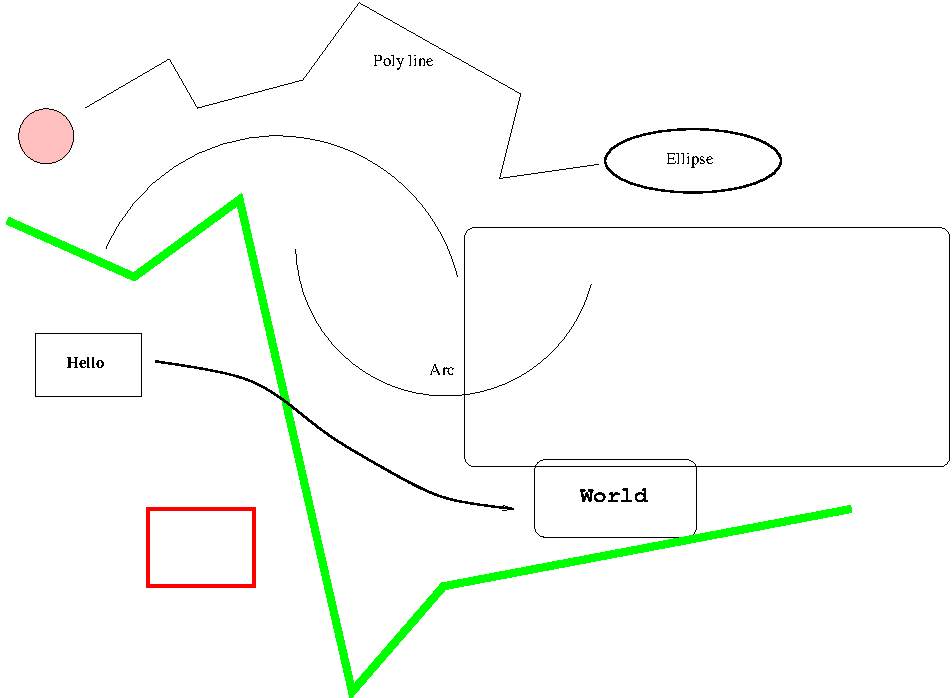
\includegraphics{figs/diagram.pdf}}
% \caption{Example diagram drawn using \texttt{xfig}}
% \label{xfig}
% \end{figure}
